%%%%%%%%%%%%%%%%%%%%%%%%%%%%%%%%%%%%%%%%%
% Beamer Presentation
% LaTeX Template
% Version 1.0 (10/11/12)
%
% This template has been downloaded from:
% http://www.LaTeXTemplates.com
%
% License:
% CC BY-NC-SA 3.0 (http://creativecommons.org/licenses/by-nc-sa/3.0/)
%
%%%%%%%%%%%%%%%%%%%%%%%%%%%%%%%%%%%%%%%%%

%----------------------------------------------------------------------------------------
%	PACKAGES AND THEMES
%----------------------------------------------------------------------------------------

\documentclass{beamer}

\mode<presentation> {
	\usepackage[utf8]{vietnam}
	\newcommand\tab[1][1cm]{\hspace*{#1}}
	\graphicspath{ {images/} }
	% The Beamer class comes with a number of default slide themes
	% which change the colors and layouts of slides. Below this is a list
	% of all the themes, uncomment each in turn to see what they look like.
	
	%\usetheme{default}
	%\usetheme{AnnArbor}
	%\usetheme{Antibes}
	%\usetheme{Bergen}
	%\usetheme{Berkeley}
	%\usetheme{Berlin}
	%\usetheme{Boadilla}
	%\usetheme{CambridgeUS}
	%\usetheme{Copenhagen}
	%\usetheme{Darmstadt}
	%\usetheme{Dresden}
	%\usetheme{Frankfurt}
	%\usetheme{Goettingen}
	%\usetheme{Hannover}
	%\usetheme{Ilmenau}
	%\usetheme{JuanLesPins}
	%\usetheme{Luebeck}
	\usetheme[secheader]{Madrid}
	%\usetheme{Malmoe}
	%\usetheme{Marburg}
	%\usetheme{Montpellier}
	%\usetheme{PaloAlto}
	%\usetheme{Pittsburgh}
	%\usetheme{Rochester}
	%\usetheme{Singapore}
	%\usetheme{Szeged}
	%\usetheme{Warsaw}
	
	% As well as themes, the Beamer class has a number of color themes
	% for any slide theme. Uncomment each of these in turn to see how it
	% changes the colors of your current slide theme.
	
	%\usecolortheme{albatross}
	%\usecolortheme{beaver}
	%\usecolortheme{beetle}
	%\usecolortheme{crane}
	%\usecolortheme{dolphin}
	%\usecolortheme{dove}
	%\usecolortheme{fly}
	%\usecolortheme{lily}
	%\usecolortheme{orchid}
	%\usecolortheme{rose}
	%\usecolortheme{seagull}
	%\usecolortheme{seahorse}
	%\usecolortheme{whale}
	%\usecolortheme{wolverine}
	
	%\setbeamertemplate{footline} % To remove the footer line in all slides uncomment this line
	%\setbeamertemplate{footline}[page number] % To replace the footer line in all slides with a simple slide count uncomment this line
	
	%\setbeamertemplate{navigation symbols}{} % To remove the navigation symbols from the bottom of all slides uncomment this line
	\setbeamertemplate{section in toc}[circle]
	\setbeamertemplate{subsection in toc}[square]
}

\usepackage{graphicx} % Allows including images
\usepackage{booktabs} % Allows the use of \toprule, \midrule and \bottomrule in tables
\usepackage{caption}
\usepackage{fancyvrb}
\usepackage{bbm}
\graphicspath{ {images/} }
\usepackage[style=authortitle,backend=bibtex]{biblatex}
\usepackage{makecell}
\usepackage{xcolor}
\usepackage{subfig}
\usepackage[export]{adjustbox}% http://ctan.org/pkg/adjustbox
\addbibresource{ref.bib}
%\everymath{\color{blue}}%make in-line maths symbols blue to read/check easily

%\sloppy
\captionsetup[figure]{labelfont={small,bf},textfont={small,it},belowskip=-1pt,aboveskip=-9pt}
\captionsetup[table]{labelfont={small,bf},textfont={small,it},belowskip=-1pt,aboveskip=7pt}

\setbeamercovered{highly dynamic}
\newcounter{saveenumi}
\newcommand{\seti}{\setcounter{saveenumi}{\value{enumi}}}
\newcommand{\conti}{\setcounter{enumi}{\value{saveenumi}}}
\resetcounteronoverlays{saveenumi}

%----------------------------------------------------------------------------------------
%	TITLE PAGE
%----------------------------------------------------------------------------------------

\title[]{ZA Seminar}


\author[]{Lê Hoàng Trung} % Your name


\institute[HCMUS] % Your institution as it will appear on the bottom of every slide, may be shorthand to save space
{
	%\bf{Đại học Khoa Học Tự Nhiên Thành phố Hồ Chí Minh} \\ % Your institution for the title page
	%\medskip
	%\bf{Khoa Công Nghệ Thông Tin}\\
	%\medskip
	\textit{le.hg.trung@gmail.com} % Your email address
}

\date[\today]{} % Date, can be changed to a custom date
\logo{
\includegraphics[height=0.65cm]{hcmus.png}}

%\AtBeginSection[]{
%	\frame{\sectionpage}
%	\begin{frame}{Mục lục}
%		\tableofcontents[currentsection, hideothersubsections]
%	\end{frame}
%}

\begin{document}
\begin{frame}[plain]
	\maketitle
	\small
	{\centering\itshape \huge{\bf{An approach for QA using dependency parsing}} \par}
	\footnotesize
	\begin{table}[c]
		\centering 
		\begin{tabular}{rrl}
			%\vspace{0.5cm}
			%\hspace{1.5 cm} & Hội đồng & : \bf{Khoa học máy tính}\\
			%	\vspace{0.5cm}
			%\hspace{1.5 cm} & Giảng viên hướng dẫn & : \bf{ThS. Trần Trung Kiên}    \\
			%\vspace{0.5cm}
			%\hspace{1.5cm} & Giảng viên phản biện & : \bf{TS. Nguyễn Đức Dũng}\\
			%\vspace{0.5cm}
			%\hspace{1.5 cm} & Sinh viên thực hiện     & : \bf{Lê Hoàng Trung - 1412587} \\
			%	\vspace{0.5cm}
			%\hspace{1.5 cm} & \hspace{5 cm} &  \hspace{0.15cm} \bf{Bùi Khánh Ngọc - 51302567}\\
							
		\end{tabular}
	\end{table}
	\begin{center}
		{\footnotesize Tp. Hồ Chí Minh, Tháng 03/2018}
	\end{center}
\end{frame}
	
%------------------------------
%\begin{frame}
%	\frametitle{Overview} % Table of contents slide, comment this block out to remove it
%	\tableofcontents[pausesections, hideallsubsections] % Throughout your presentation, if you choose to use \section{} and \subsection{} commands, these will automatically be printed on this slide as an overview of your presentation
%\end{frame}
%---------------------------------
	
%----------------------------------------------------------------------------------------
%	PRESENTATION SLIDES
%----------------------------------------------------------------------------------------
	
	
\section{Question Answering}
\begin{frame}
	\frametitle{Question Answering}		
		
		
		\begin{center}
			\centering
				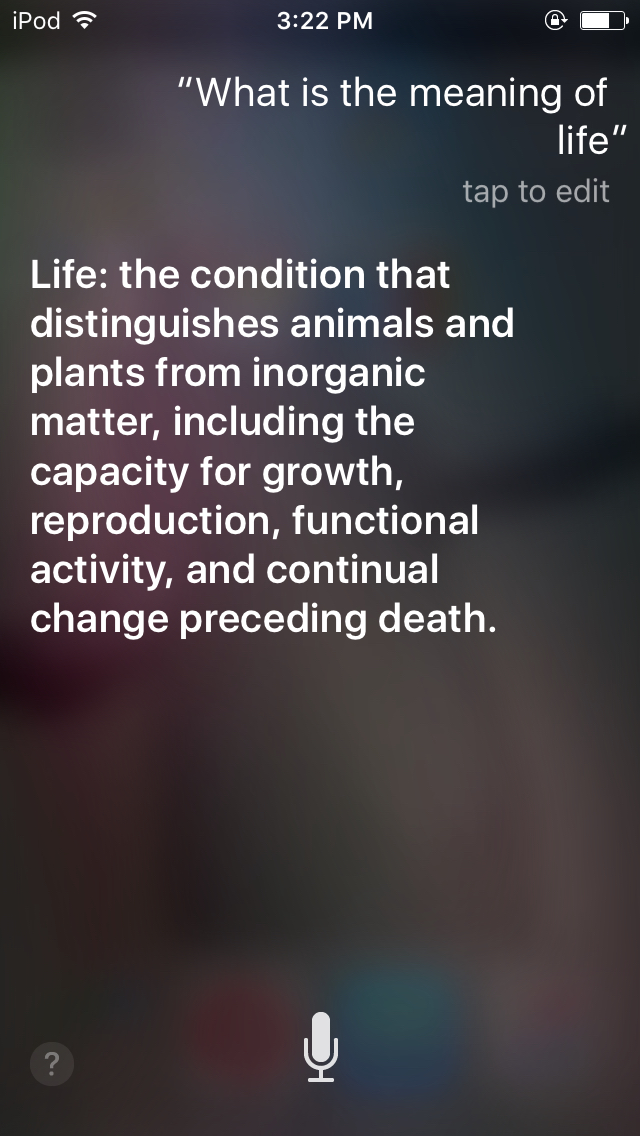
\includegraphics[width=\textwidth,height=0.8\textheight,keepaspectratio]{siri}
				\vspace{0.5cm}
		\end{center}			
		
			
\end{frame}
	
\begin{frame}
	\footnotesize
	\frametitle{Type of Questions}
			
	\begin{itemize}
		\item[•] Factoid questions
			\begin{itemize}
				\item[•] Who is Putin?
				\item[•] How much water should a person drink a day?
				\item[•] Who wrote the book forrest gump was based on?
				\item[•] Does C++11, 14, 17 or 20 introduce a standard constant for pi?
			\end{itemize}
		
		\item[•] Non-factoid questions
			\begin{itemize}
			\item[•] What is the meaning of life?
			\item[•] Does writing matter a lot in research?
				\item[•] How can I give out my telephone number to my neighbors without implying anything?
			\end{itemize}
	\end{itemize}
			
\end{frame}


\begin{frame}
	\frametitle{Approaches for QA}		
			
	\begin{itemize}
		\item[•] Information Retrieval approaches
			\begin{itemize}
				\item[•] Answer the question based on textual data.
				\item[•] Given a question, IR systems find out the paragraph that answer for it.
			\end{itemize}
	\end{itemize}		
		
			
\end{frame}


\begin{frame} 
	\frametitle{Information Retrieval approaches} 
	\begin{center} 
		\centering 
			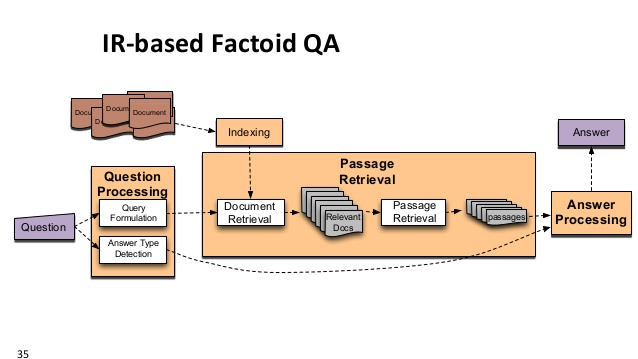
\includegraphics[width=\textwidth,height=\textheight,keepaspectratio]{irbase} 			
			\vspace{0.5cm} 
	\end{center} 
\end{frame} 

\begin{frame} 
	\frametitle{Information Retrieval approaches} 
	Q: \textit{Which US state capital has the largest population?} 
	\begin{itemize} 
		\item \textbf{Answer Type:} city 
		\item \textbf{Query:} US state capital, largest, population 
		\item \textbf{state captital} 
	\end{itemize} 
\end{frame} 

\begin{frame}
	\frametitle{Approaches for QA}		
		
	\begin{itemize}
		\item[•] Knowledge-based and Hybrid approaches
			\begin{itemize}
			\item[•] We convert the question into a semantic representation (kind of SQL queries).
			\item[•] Ex: \textit{"What countries has population over 100 milions?"} $\Rightarrow$ \textit{SELECT country.name FROM country WHERE country.population > $10^9$}
			\end{itemize}
	\end{itemize}		
		
\end{frame}


\begin{frame}
	\frametitle{Approaches for QA}		

			
	\begin{itemize}
		\item[•] Information Retrieval approaches
			\begin{itemize}
			    \item[•] Based on retriving and reranking documents.
				\item[•] Easier to implement.
				\item[•] Not precise comparing to KB
				\item[•] We don't understand the meanning of the questions.
			\end{itemize}
		
		\item[•] Knowledge-based and Hybrid approaches
			\begin{itemize}
			\item[•] Base on exact queries over a structured database.
			\item[•] Hard to implement (of course).
			\item[•] Precise
			\item[•] Help us understand the \textbf{semantic meaning} of the questions. 
			\end{itemize}
	\end{itemize}		
		
			
\end{frame}


\begin{frame}
	\frametitle{Dependency parsing}
			
	\begin{center} 
		\centering 
			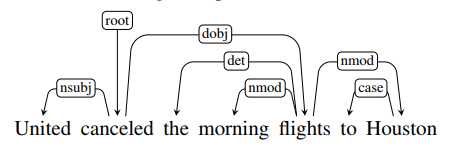
\includegraphics[width=0.7\textwidth,height=0.7\textheight,keepaspectratio]{example} 			
			\vspace{0.5cm} 
	\end{center}		
		
\end{frame}

\begin{frame}
	\frametitle{Dependency parsing}
	
	Type of Dependencies
	\begin{center} 
		\centering 
			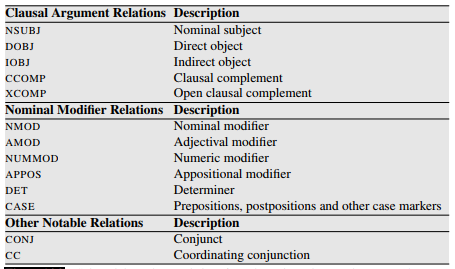
\includegraphics[width=0.7\textwidth,height=0.7\textheight,keepaspectratio]{dptypes} 			
			\vspace{0.5cm} 
	\end{center}	
		
\end{frame}

\begin{frame}
	\frametitle{Dependency parsing}
	
	Properties of dependency tree
	\begin{itemize}
		
		\item[•] There is a single designed root node that has no incoming arcs.
		\item[•] With the exception of the root node, each vertex has exactly one incoming arc.
		\item[•] There is a unique path from the root node to each vertex in $V$.
		\item[•] Dependency tree is projective.		
		
	\end{itemize}		
		
\end{frame}

\begin{frame}
	\frametitle{Dependency parsing}
			
	\begin{center} 
		\centering 
			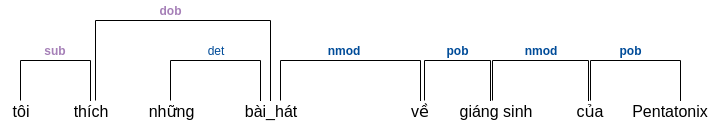
\includegraphics[width=\textwidth,height=\textheight,keepaspectratio]{qa_first_ex} 			
			\vspace{0.5cm} 
	\end{center}		
		
\end{frame}

\begin{frame}
	\frametitle{Proposed method}
			
	\begin{center} 
		\centering 
			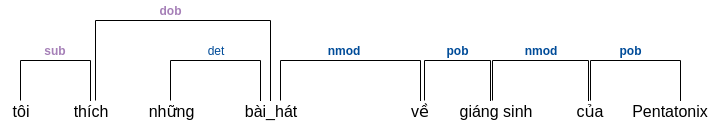
\includegraphics[width=\textwidth,height=\textheight,keepaspectratio]{qa_first_ex} 			
			\vspace{0.5cm} 
	\end{center}		
		
\end{frame}
	
\section{Tham khảo}
\begin{frame}
	\frametitle{Tham khảo}
	\printbibliography
\end{frame}
	
	
%------------------------------------------------
	
	
	
	
	
\end{document}